\documentclass{beamer}

\usepackage{beamerthemesplit}
\usepackage{latexsym}
\usepackage{eurosym}
\usepackage[activeacute,spanish]{babel}
\usepackage{ae,aecompl}
\usepackage{graphicx}
\usepackage{amsfonts}
\usepackage{float}

\usetheme{Darmstadt}

\title{Marsans Argentina}
\author{ Grupo R2 }
\date{\today}

\begin{document}

\frame{\titlepage}

\section[�ndice]{}
\begin{frame}[allowframebreaks]
\tableofcontents
\end{frame}
%\frame{\tableofcontents}
		
		
\section{Informacion General de la Empresa}
	
	\begin{frame}
	%\frametitle{Escenario Previo.}
	
	\begin{figure}[H]
	\centering
	\includegraphics[scale=0.4]{Imagenes/logo.jpg} 
	\end{figure}		
	
	
	\end{frame}
	
	%\subsection{Historia de la empresa}
	\begin{frame}%[allowframebreaks]
	\frametitle{Historia de la empresa}		
		\begin{itemize}
			\item Marsans internacional es fundada  en 1908 en la ciudad de Barcelona,  Espa\~na.
			\pause
			\item Comienza siendo una empresa viajes y turismo minorista.
			%\uncover<3> {\item Comienza siendo una empresa viajes y turismo minorista.}
			
			\pause
			\item Con los a\~nos comienza a expandirse por el mundo, fundando filiales.
			\pause
			\item Llega a la Argentina y comienza a tener mucho exito. Este llega a su pico maximo durante el periodo de convertibilidad.
			\pause
			\item En los ultimos a\~nos, mas precisamente en el 2008, Marsans Argentina atraviesa una crisis, la cual pone en jaque su existencia.
		\end{itemize}
	\end{frame}	

	\begin{frame}
	\frametitle{Organigrama de la Empresa}
	
		\begin{figure}[H]
		\centering
		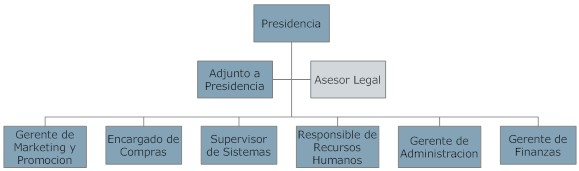
\includegraphics[scale=0.5]{Imagenes/organigramaViejo.jpg} 
		\end{figure}		
	
	
	\end{frame}
	
\section{Problemas identificados}
		\begin{frame}%[allowframebreaks]
		\frametitle{Dise�o y Cambio Organizacional}		
			
			\begin{block}{\uncover<1->{Necesidad de Reestructuracion}}
				
				\uncover<2->{
				\begin{itemize}
					\item Estrato dirigencial sobredimensionado.
					\item Estructura inadecuada luego de importantes recortes de personal
					\item Incertidumbre de los empleados en cuanto a las funciones que deben desempe�ar

				\end{itemize}
				}
			
			\end{block}
				
			\begin{block}{\uncover<1->{Manejo Departamental}}
				\uncover<3->{
				\begin{itemize}
					\item Falta de comunicaci�n y colaboracion entre las distintas �reas y utilizaci�n de canales informales
				\end{itemize}
				}
				
			\end{block}
			
			\begin{block}{\uncover<1->{ Falta de Confianza en la direccion General}}
				\uncover<4->{
				\begin{itemize}
					\item Falta de conducci�n y estrategia indefinida
				\end{itemize}
				}
			
			\end{block}
			
		\end{frame}	
	
		\begin{frame}%[allowframebreaks]
		\frametitle{Ingenieria del Producto}		
			\begin{block}{\uncover<1->{ Problemas  para generar valor agregado}}
				\begin{itemize}
					\uncover<2->{
					\item No se utilizan los resultados de Investigaciones de Marketing.
					\item Falta de integraci�n entre los trabajos de distintos departamentos
					}
				\end{itemize}
			
			\end{block}	
				
			\begin{block}{\uncover<1->{ Malas inversiones comerciales}}
				
				\begin{itemize}
					\uncover<3->{
					 \item Esfuerzos dispersos en demasiados productos
					}
				\end{itemize}
				
			\end{block}		
				
			\begin{block}{\uncover<1->{ Falta de flexibilidad Frente a las fluctuaciones del mercado.}}
				\begin{itemize}						
					\uncover<4->{
					\item No se implementaron cambios en los productos ofrecidos a pesar de la crisis.
					}
				\end{itemize}		
			\end{block}			
			
		\end{frame}	
	
		\begin{frame}%[allowframebreaks]
		\frametitle{Marketing}		
			\begin{block}{ Imagen Comercial}	
				
					 Mal concepto de la empresa luego del esc�ndalo de
 Aerol�neas Argentinas	
				
			\end{block}
			
			\begin{figure}[H]
			\centering
			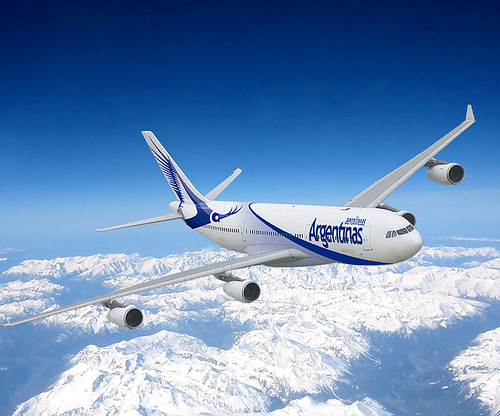
\includegraphics[scale=0.32]{Imagenes/viajeMarketing.jpg} 
			\end{figure}		
	
		\end{frame}	
	
		\begin{frame}%[allowframebreaks]
		\frametitle{Inestabilidad Financiera}		
			\begin{block}{Atraso en el pago de sueldos.}
					 Disconformidad de los recursos				
			\end{block}	
			\pause
			
			\begin{block}{Despidos masivos para reducir costos.}
					Incertidumbre,  falta de entusiasmo y responsabilidad	
			\end{block}		
				
		\begin{figure}[H]
		\centering
		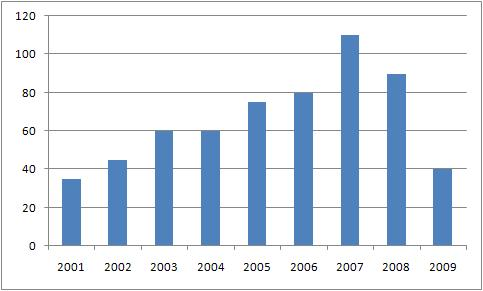
\includegraphics[scale=0.40]{Imagenes/EmpleadosEfect.jpg} 
		\caption{Empleados Efectivos}
		\end{figure}		
		
		\end{frame}	
	
	\section{Propuesta de Cambio}
		\begin{frame}%[allowframebreaks]
		\frametitle{Estrategia Propuesta}		
			\begin{itemize}
				\item Reducir la estructura de la empresa.
				\pause
				
				\item Centrar a la empresa en pocos productos.
				\pause
				\item Motivar al personal.
				\pause		
				\item Redistribuir la fuerza de trabajo entre las distintas �reas.
				\pause
				\item Evitar la p�rdida de personal con inducci�n y la contrataci�n de personal poco capacitado y/o sin experiencia.
			\end{itemize}
		\end{frame}	
		
		
			\begin{frame}%[allowframebreaks]		
			\frametitle{Organigrama de la Empresa}
				\begin{figure}[H]
				\centering
				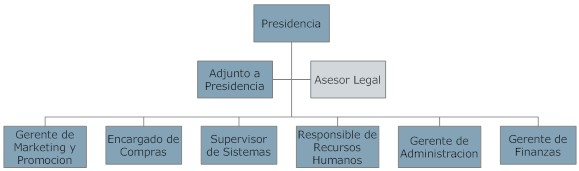
\includegraphics[scale=0.5]{Imagenes/organigramaViejo.jpg} 
				\end{figure}		
			\end{frame}
			
			\begin{frame}[allowframebreaks]		
			\frametitle{Propuestas respecto el dise\~no organizacional}
				
					\begin{figure}[H]
					\centering
					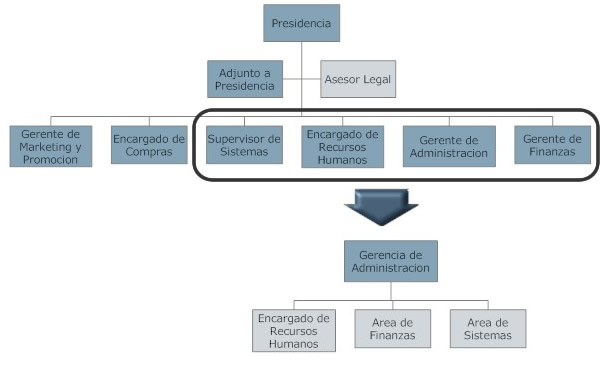
\includegraphics[scale=0.35]{Imagenes/orgCambio1.jpg} 
					\caption{Fusi\'on de las gerencias y areas de Administracion, Sistemas, Finanzas y Recursos Humanos}
					\end{figure}		

					\begin{figure}[H]
					\centering
					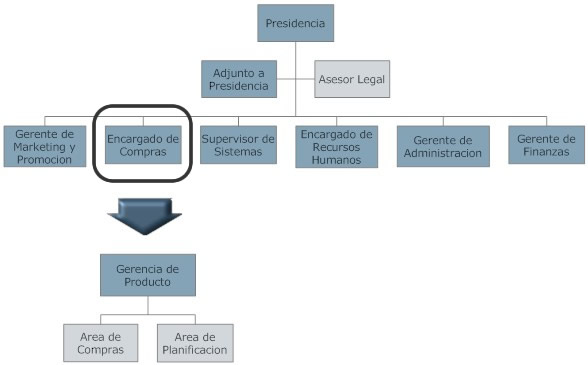
\includegraphics[scale=0.35]{Imagenes/orgCambio2.jpg} 
					\caption{Creaci�n de una Gerencia de Producto que abarca las �reas de Planificaci�n y compras.}
					\end{figure}		

					\begin{figure}[H]
					\centering
					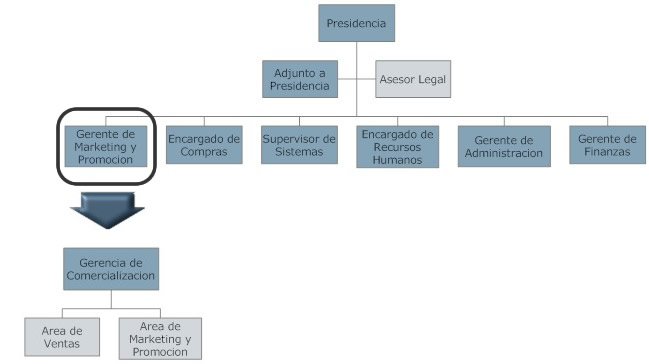
\includegraphics[scale=0.35]{Imagenes/orgCambio3.jpg} 
					\caption{Creaci�n de una Gerencia de Comercializaci�n que nuclea el �rea de Marketing y Promoci�n y la de Ventas.}
					\end{figure}		
 			

					\begin{figure}[H]
					\centering
					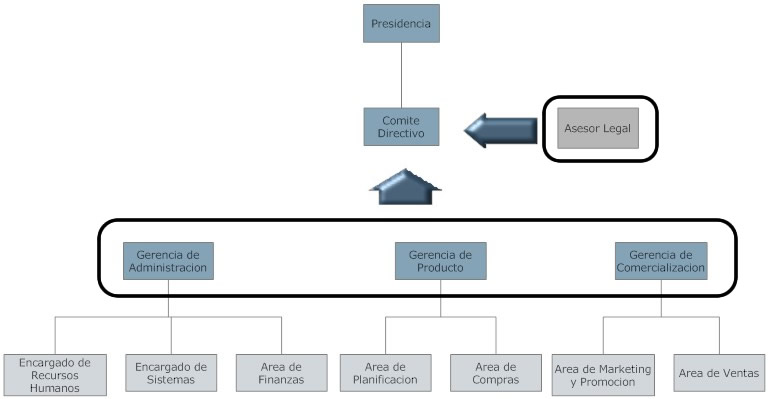
\includegraphics[scale=0.30]{Imagenes/orgCambio4b.jpg} 
					\caption{Creaci�n de un Comit� Directivo para mejorar el proceso de toma de decisiones. El Asesor Legal esta vinculado con el comit�,  perdiendo comunicaci�n directa con la presidencia.}
					\end{figure}							
				
			\end{frame}

			\begin{frame}%[allowframebreaks]		
			\frametitle{Organigrama Propuesto para la Empresa}
				\begin{figure}[H]
				\centering
				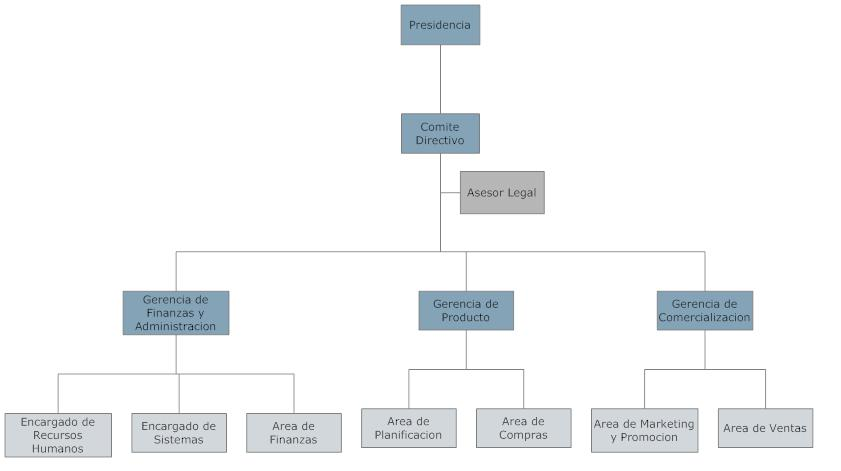
\includegraphics[scale=0.40]{Imagenes/organigramaNuevo2.jpg} 
				\end{figure}		
			\end{frame}
	
			\begin{frame}%[allowframebreaks]		
			\frametitle{Cambios no estructurales propuestos }
			
				\begin{block}{\uncover<1->{Ingenier\'ia de Producto}}
					\begin{itemize}
						\uncover<2->{
						\item Integraci\'on del trabajo del area de ventas y del de Marketing y promoci\'on dentro de la Gerencia de Comercializaci\'on.						
						\item An�lisis intensivo de mercado para crear nuevos productos.

						\item Concentrar esfuerzos en pocos productos
						}
					\end{itemize}
				\end{block}	
					
				\begin{block}{\uncover<1->{Imagen Comercial.}}
					\begin{itemize}
						\uncover<3->{
						\item Cambio de nombre de la empresa.
						}
					\end{itemize}
				\end{block}	

			\end{frame}
	
	\section{Conclusiones}
		\begin{frame}
		\frametitle{Conclusiones}
			\begin{enumerate}
				
				% Estructura consistente en teoria y en practica.  
				\item {Consistencia}
				\pause
				
				% Dinamica. 
				% La estructura tiene que poder adaptarse rapidamente a los cambios que sufre la organizacion.
				\item {Dinamismo}
				\pause
				
				% Motivacion.
				% La organizacion debe prestarle atencion a la motivacion de los empleados ya que ellos son el capital mas grande de la empresa. 
				\item {Motivaci\'on}
				\pause
				
				%Planeamiento.
				% La organizacion debe tener siempre una vision a futuro que le permita ... :p
				\item {Planeamiento}
				
			\end{enumerate}
		\end{frame}
\end{document}